\chapter{Un fruit du « pré-réformisme » : le wahhabisme}
\mn{ \emph{(31/01/2022)}}

%---------------------------------------------------------
\section{Le wahhabisme}
\paragraph{Pourquoi en parler} C'est un courant qui a presque trois siècles, avec une évolution dans le monde du musulman qui a évolué. Il faut penser l'Islam contemporain dans son contexte.

 
  \subsection{Muhammad Ibn al Wahhab
  (1702-1792)} 
  \label{Theol:AlWahhab}
  
\paragraph{Origine} Son père est \emph{qadi}\sn{juge} et enseignant. Dans le Hadz. Fait un pélerinage à la Mecque. Renouveau

\paragraph{Formation et premières prédications} Proclame le \emph{Tawhid} l'unicité et lutte contre toutes les pratiques "déviantes". Il se heurte aux autorités locales et retourne donc à la Mecque. Il se forme là avec des maîtres d'Arabie et Indien. Puis se rend à Basra, à un autre maître. C'est là qu'il rencontre les si'ites. Il se heurte de nouveau aux autorités locales. Il rentre en Arabie mais \textit{son père y est hostile}. Ce n'est pas un grand savant mais un lettré. 
 
\paragraph{L'alliance avec Ibn Se`ud} Alliance matrimoniale avec un chef de tribu de la Mecque. Il se rend indésirable et il est obligé de partir et il arrive dans le village de Dariya et il y rencontre un autre chef de village, Mohammed Ibn Se'ud, alliance elle aussi politicolo-religieuse et matrimoniale en 1744. Ibn Se'ud accepte la doctrine et al Wahhab légitime l'acquisition de terre par Ibn Se'ud. 

Wahhab enseigne beaucoup  : il écrit beaucoup à des savants (\emph{Oulema}) à l'intérieur et l'extérieur du royaume de Ibn Se'ud. \textit{selon un modèle prophétique}, Mohammad ayant écrit au Basileos,... 

\paragraph{Un développement politique} Conquiert toute l'Arabie Saoudite. En 1818, c'est la fin du premier état wahhabite car l'empire ottoman intervient et execute le fils de Ibn Se'ud.
    
 Il s'appuie sur deux auteurs : 
\begin{itemize}
    \item Ibn Taymiyya (1263-1328), \label{Theol:Taymiyya2} \sn{cf p. \pageref{ibn-taymiyya}}, un vrai penseur
    \item Ibn Qayyim (1292-1350) un de ces disciples
\end{itemize}
 
Ibn Wahhab insiste sur le retour à la source mais en fait il lit le Coran à travers ces deux auteurs.

\paragraph{Une doctrine condamnée} Son père et son frère s'opposent à lui. Une fatwa contre lui du fait de sa critique sur les différentes écoles juridiques et le fait qu'il exclut de la communauté musulmanes ceux qui ne pensent pas comme lui. 

  \subsection{La doctrine wahhabite} 



  \paragraph{Nécessité du retour aux sources} Accentuation des sources, bien sûr le Coran. 
  \begin{itemize}
      \item  \item  Wahhab s'éloigne d'une lecture du Coran ligne à ligne mais propose une analyse \textit{thématique}.
  \item Il rejette aussi le besoin d'une \textit{médiation} humaine pour comprendre le Coran. Il s'oppose aux \emph{Ashraf}, les descendants du prophète \sn{Les Ashrafs ont un statut particulier dans l'Islam} ainsi qu'aux \emph{Imams} dans le si'isme, ainsi que les \emph{sheykhs} soufis.
  \begin{Prop}
  Il n'y a pas besoin de sciences particulières pour accéder au sens du Coran, d'après Wahhab. 
  \end{Prop}
  \item il suis les \emph{Hadiths}, la seule exégèse possible, la \textit{sunna} et rejette les grands commentaires classiques du Coran.  Cela va jusqu'à critiquer la tradition des 4 premiers Califes \textit{bien guidés}. Abu Bakr avait détourné la \textit{zakat} pour ses propres dépenses.
  \item Il reprend la distinction d'Ijtihad, qu'il limite aux versets aux versets obscures, contre le taqlid. Il s'oppose à deux principes de l'Ijtihad : qiyas (recours par analogie : alcool et drogue), \textit{ijama} (consensus des savants : on considère que cela fait autorité \sn{Infaillabilité de la communauté dans les Hadiths}), et le \textit{ra'y}, l'opinion personnelle du juriste. 
  
  \end{itemize}
 
 \begin{Prop}
 Il conteste les principes sous-jacents aux savants qui l'ont précédés. Il y a une tension entre son ambition de revenir au Coran mais en parallèle en se mettant en filiation avec Ibn Taymiyya
 \end{Prop}
 
 
  \paragraph{Une notion centrale : le \emph{tawhid} (unicité divine)}
  
  \mn{{Extraits du \emph{Kitab at-tawid} (Livre de
l'unicité divine) de Muhammad Ibn Wahhab} . {Chapitre 1} : \emph{Tawhid}
Traduction et édition établies en Arabie Saoudite. Allah est traduit par Allah et non Dieu, alors qu'en Arabe, Dieu est traduit par Allah y compris pour les chrétiens arabes. }

\begin{quote}
\emph{Allah-ta`ala} a dit : « Je n'ai créé les djinns et les hommes que
pour qu'ils M'adorent (1 :56)\ldots Et très certainement nous avons
suscité dans chaque communauté un message pour leur dire d'adorer Dieu
et d'écarter le Rebelle (16 :36)\ldots Et voilà que ton Seigneur a
décrété que tu dois n'adorer que Lui et faire preuve de bonté envers tes
parents (17 :23)\ldots Adorez Dieu et ne lui donnez quelque associé que
ce soit (4 :36)\ldots Venez, je vais vous réciter ce que votre Seigneur
vous a interdit ; - ceci : Ne lui associez quoi que ce soit\ldots(6
:151-153) ». Ibn Mas`ud a dit : « Quiconque se propose de vérifier le
testament du Prophète Muhammad (SWA) -- un testament sur lequel le
Prophète a apposé son sceau, qu'il lise ces mots d'Allah : « Venez, je
vais vous réciter ce que votre Seigneur vous a interdit ; - ceci : Ne
lui associez quoi que ce soit\ldots Voilà ce qu'il enjoint » (6 :
151-153)


Mu`adh Ibn Jabal raconta : « Je montai derrière le Prophète (SAW) quand
il me dit : « Ô Mu`adh ! Sais-tu ce que les créatures d'Allah Lui
doivent et ce qui leur est dû ? » Je répondis : « Allah et son Prophète
savent mieux ». Il continua : « Ce que les créatures d'Allah Lui
doivent, c'est de ne jamais associer qui que ce soit avec Lui. Ce qui
leur est dû, c'est qu'il ne punira aucune personne qui ne Lui associe
pas un autre ». Je dis :

« Ô Prophète d'Allah, est-ce que je peux annoncer la bonne nouvelle aux
gens ? » Il répliqua : «Non ! Ne leur dis rien de peur qu'ils comptent
sur la promesse et manquent à leurs devoirs envers Lui». Ce hadith est
mentionné dans deux \emph{Sahihs}.


D'autres points :


\begin{enumerate}

\item
  \begin{quote}
  La sagesse dans la création du djinn et de l'humanité.
  \end{quote}
\item
  \begin{quote}
  Le service à Allah consiste en le \emph{tawhid}. Car, à l'opposé du
  \emph{tawhid} se trouve l'aliénation d'Allah. (\ldots)
  \end{quote}
\item
  \begin{quote}
  La sagesse d'envoyer des prophètes. (\ldots)
  \end{quote}
\end{enumerate}
  \end{quote}
  
On trouve une accumulation de versets coraniques sur le thème, puis des hadiths du prophète. Le grand péché par excellence, c'est le \emph{shirk}, l'associationisme des Dieux à Dieu. Or Wahhab va plus loin. 

\begin{quote}


\emph{Allah-ta`ala} dit : « Ceux qui ont cru et n'ont point revêtu de
prévarication leur foi\ldots{} » (6 : 82).

(\ldots) Abu Sa`id al Khudriyy rapporta que le Prophète d'Allah (SWA) a
dit : « Quand Musa {[}Moïse{]} demanda à Allah de lui enseigner une
prière qu'il puisse réciter à chaque fois qu'il pensait à Lui ou qu'il
L'évoquait, Allah répondit : « Dis, ô Musa, qu'il n'y a d'autre Dieu
qu'Allah. Musa dit : « Ô Seigneur, tous tes serviteurs prononcent ces
mots ». Allah dit : « Ô Musa, si les sept cieux et tout ce qu'ils
renferment, et les sept terres aussi, si tout cela était pesé contre
cette phrase : « Il n'y a d'autre Dieu qu'Allah », cette dernière
pèserait plus lourd ». Ibn Hibban rapporta cela également et al-Hakim
compléta sa version. Al-Tirmidhi enregistra, avec peu de rédaction, le
récit de Anas à l'effet qu'il entendit le Prophète d'Allah (SWA) dire :
« Allah dit : « Ô Homme ! Si tu venais à Moi avec tous les sacs du monde
remplis de tes péchés, mais avec le témoignage que tu n'associes rien à
Moi, Je viendrais à toi avec tous mes sacs remplis de miséricorde et de
pardon ! ».

    
\end{quote}

\begin{Synthesis}
Si on respecte le \emph{Tawhid}, cela suffit à pardonner les péchés, mais important de respecter les principes de l'Islam (c'est pour cela que c'est caché)
\end{Synthesis}

\paragraph{Distinction au sein du Tawhid } 
\begin{Def}[Le grand Shirk ]
Il distingue le \emph{tawhid rububiyya} (l'unicité de souverainté du monde) avec le \emph{tawhid uluhiyya} (de divinité) : ne reconnaitre aucun intermédiaire entre Dieu et les hommes. Il ne peut y avoir de dévotion que pour Dieu seul : les saints, les soufis, les Imams.
\end{Def} 
Al Wahhab introduit une critique fondamentale contre le soufisme. 

\paragraph{Le petit Shirk} 
\mn{{Chapitre 4} : La crainte du \emph{shirk}}
\begin{quote}
Allah -- qu'Il soit loué et glorifié -- dit : « Non, Dieu ne pardonne
pas qu'on Lui donne quelque associé. En deçà, Il pardonne à qui il veut
» (4 : 48, 116)

(\ldots) Dans le hadith, nous lisons : « Ce que je crains le plus pour
vous, c'est le moindre \emph{shirk}. Quand on lui demanda ce que
c'était, le Prophète répondit : « l'hypocrisie ». Dans le Sahih
d'al-Bukhari, nous lisons que Ibn Mas`ud reporta : « Le Prophète d'Allah
(SWA) a dit : « Celui qui rencontre Allah le jour du Jugement sans Lui
avoir associé qui que ce soit ira au Paradis, et celui qui le rencontre
ayant fait le contraire sera consigné en Enfer ».
\end{quote}
\begin{Def}[le Petit Shirk]
Toute attitude de l'homme qui ne sert pas Dieu. il relève aussi de l'attitude morale.
\end{Def}

\begin{Ex}[L'appel à témoigner qu'il n'y a d'autre
Dieu qu'Allah]

\mn{{Chapitre 5} : }
\begin{quote}
\emph{Allah-ta`ala} a dit : « Dis (ô Muhammad) : `\,`Voici mon sentier,
j'appelle à Dieu'\,' » (12 :108)

Ibn `Abbas (RA) rapporta : « Quand le Prophète d'Allah (SAW) envoya
Mu'adh à al-Yaman, il lui recommanda : `\,`Quand tu rencontres des gens
du Livre, que ta première action soit de leur demander de témoigner
qu'il n'y a d'autre Dieu qu'Allah'\,' ». Selon un autre récit, «
\ldots{} de leur demander de réaliser l'unicité d'Allah. S'ils
t'obéissent, informe-les qu'Allah leur a imposé la \emph{salat} cinq
fois par jour. S'ils t'obéissent en cela, alors informe-les qu'Allah
leur a imposé le devoir de charité qui doit être perçue des riches pour
être distribué aux pauvres. S'ils t'obéissent en cela, ne touche pas à
leurs autres biens et occupe-toi de la plainte de l'opprimé, car il n'y a aucun obstacle dans son accès à Allah ».
(Rapporté dans les \emph{Sahihs} d'al-Bukhari et de Muslim). (\ldots)
\end{quote}
\end{Ex}



\paragraph{Les Intercessions} L'intercession est limitée à Mohammed, et uniquement aux musulmans suivants Wahhab. On ne peut pas prier le Prophète. Peut être intervient-t-il au jugement dernier.


\mn{{Chapitre 17} : L'intercession}
\begin{quote}
Allah -- qu'il soit loué et glorifié -- a dit : « Et par ceci (le
Qur'an), avertis ceux qui, n'ayant pour eux hors de Dieu, ni ami ni
intercesseur, craignent d'être rassemblés vers le Seigneur\ldots{} » (6
: 51). Dis : « A Dieu l'intercession tout entière\ldots{} » (39 : 44).
Qui peut intercéder auprès de Lui que par sa permission ?... (2 : 255).
Et combien d'anges dans les cieux ? Leur intercession ne met au large en
rien, sauf après que Dieu l'a permis, en faveur de qui il veut et qu'il
agrée » (53 : 26). (\ldots)

(\ldots) En tant que catégorie générale du Jour du Jugement en laquelle
les mécréants croient, l'intercession est rejetée par le Qur'an. Le
Prophète (SAW) nous informa qu'en ce jour « il sera amené devant Allah.
Il se prosternera lui-même et louera Allah, plutôt que de demander à
intercéder. Alors on lui dira : « Lève-toi ! Parle maintenant et tu
seras entendu ! Demande et il te sera donné ! Intercède et il te sera
accordé ! » (\ldots) L'intercession est donc là pour les croyants
sincères et candides. Elle n'est accordée que par la permission d'Allah
et n'appartient pas aux associationistes. (\ldots)
\end{quote}


\paragraph{Tombe du juste}
Condamnation de celui qui invoque Dieu
auprès de la tombe du juste et, a fortiori, de celui qui invoque ce
dernier.
\begin{Ex}[Un exemple de Grand Shirk]
\mn{{Chapitre 20} : Condamnation de celui qui invoque Dieu
auprès de la tombe du juste et, a fortiori, de celui qui invoque ce
dernier.}
\begin{quote}
Dans le \emph{Sahih}, A'ishah (RAA) rapporta : « Umm Salmah raconta au
Prophète d'Allah (SAW) qu'elle avait vue une église remplie d'images et
de statues en Abyssinie. Le Prophète dit : « Ceux-là sont les pires de
tous les hommes : lorsqu'un membre juste et vertueux de leur groupe
meurt, ils bâtissent une église sur sa tombe et y installent toutes
sortes d'images pour lui. Ils sont coupables de deux méfaits : celui
d'invoquer quelqu'un auprès d'une tombe et celui d'installer des images
». (\ldots)

Ainsi le Prophète interdit cette pratique et condamna celui qui la
suivait. Faire le \emph{salat} sur une tombe est également interdit,
même si aucune mosquée n'a été construite sur l'emplacement. Telle est
la signification de la déclaration suivante : « On craignait qu'elle ne
soit prise pour une mosquée ». Les Compagnons n'étaient pas supposés
construire une mosquée autour de la tombe du Prophète. Tout endroit
destiné au \emph{salat} ou tout endroit où le \emph{salat} est accompli,
est une mosquée. Tel l'a déclaré le Prophète (SAW) : « Toute la terre
est pour moi une mosquée, un endroit pur (pour accomplir le
\emph{salat}) ».
\end{quote}

\end{Ex}


  \paragraph{La question du \emph{jihad}} La question de la violence chez Wahhab. Il faut repartir de la position kharijite. Un calife doit respecter la religion de façon exemplaire. s'il ne le fait pas, il est \emph{Takfir}, mécréant. Or la vision sunnite a jugé que c'est Dieu uniquement qui jugera si un musulman est un non-musulman. Ibn Taymmayyia s'élève contre les souverains Mongols : : les souverains mongols sont certes musulmans puisqu'ils ont adopté la foi musulmane mais en surface.  Wahhab va reprendre ce concept et ceux qui n'adhèrent par au \emph{shirk} sont apostats. Un germe de violence.
  
  \begin{Synthesis}
  On voit donc l'extension du concept de Ibn Taymmayyia sur le Takfir à tout le shirk, et donc en pratique en non respect du wahhabisme.
  \end{Synthesis}
 
 Mais il n'y a pas de volonté de jihad dans le wahhabisme. On peut même faire des traités avec des non-musulmans.
 
  \section{Le devenir du wahhabisme} 
 
  
 

% ------------------------------ 
\subsection{Les trois Etats Saoudiens} 

 
  {\paragraph{1744 -1818}: une première expansion}
 
 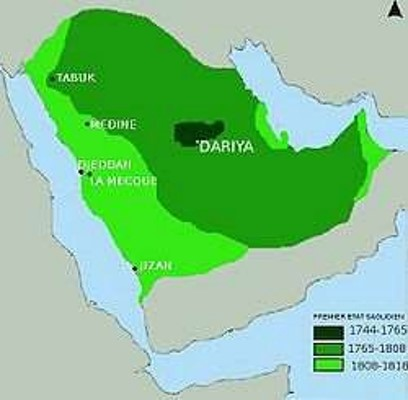
\includegraphics[width=\textwidth]{CourantsIslamContemporain/ImagesCourantsIslamContemporain/Wahhabisme1.jpg}
\emph{1744} alliance Ibn Se`ud /Ibn al-Wahhab
 
\emph{1786} conquête du Najd (`Abd-al-`Aziz)
 
\emph{1792} mort d'Ibn al-Wahhab
 
\emph{1806} conquête de La Mecque
 
\emph{1818} défaite devant les Ottomans
 

 
  {\paragraph{1821-1883}: petit Etat centré sur Riyad (Najd)}
 
  {\paragraph{1901- 2011} : le Royaume d'Arabie Saoudite} Un descendant de Wahhab qui repasse alliance avec la famille de Se'ud et conquiert l'Arabie. 
 
 
\emph{1924} conquête de La Mecque. Abdelaziz Ibn Se`ud prend le titre de
roi et \textit{protecteur des lieux saints}. On détruit les confrérie, on contrôle le pélerinage, on supprime les autres écoles de droit.

\mn{REVOIR}

\emph{1939} début de la production pétrolière \emph{1962} création de la
Ligue islamique \emph{1990} début de la guerre du Golfe.
 

 
\subsection{L'Arabie Saoudite et l'économie
pétrolière} 
 
\paragraph{ {Début de la
production}} 

\begin{quote}
1935: premier forage

1939: premier baril de pétrole

⇒ Cartel américain: l'ARAMCO
\end{quote}

 
\paragraph{{Nationalisation de la
production}}


1973: l'Etat s'approprie 25 \% des droits de l'ARAMCO (1974 : 60\%, 1980 : 100\%)


⇒ Saoudi ARAMCO: 95 \% de la production du pays.

 
\paragraph{Evolution du cours du
pétrole} 

\begin{quote}
1973: premier choc pétrolier (guerre de Kippour) =\textgreater{} de 4 à
15 \$/B

1981-1983: deuxième choc pétrolier (Révolution iranienne + guerre
Iran-Irak) =\textgreater{} 36 \$/B 2006-2008: troisième choc pétrolier
(guerre en Irak) =\textgreater142 \$/baril
\end{quote}

\paragraph{{Rente}}: 1973-2002 =\textgreater{} 200 000 milliards
de dollars au total
 
    Une étude de cas : le wahhabisme en Afrique de l'Ouest
    
\subsection{Le wahhabisme et l'Etat saoudien}

Le wahhabisme accepte une certaine ouverture en Arabie en contrepartie de financement extérieur. On est dans des \textit{concessions} des oulemas. 

\paragraph{La ligue islamique 1962} on étudie gratuitement à la Mecque et à Médine pour propager le wahhabisme.

 
\subsection{Une étude de cas : le wahhabisme en Afrique de l’Ouest}
 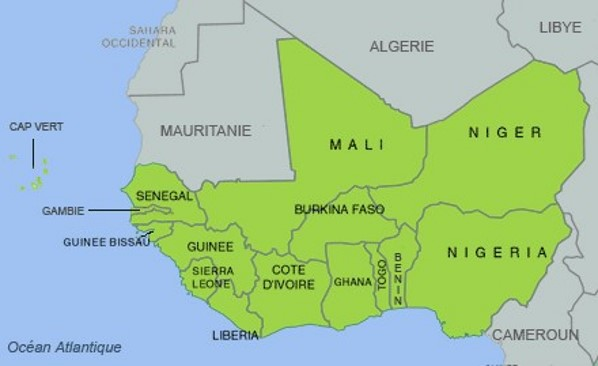
\includegraphics[width=\textwidth]{CourantsIslamContemporain/ImagesCourantsIslamContemporain/WahhabismeAfricain.jpg}
\paragraph{Des étudiants revenant de la Mecque dans les années 40} et surtout depuis dans les années 70, avec la ligue islamique. 

\paragraph{Un conflit avec les structures soufis}, maraboutisme, très puissantes. On ne priait pas dans les mêmes lieux de culte. 1978 : On  est  loin de  l'époque  où,  en  1978,  Yao  Koum  expliquait  au  Ministre  de  l'Intérieur  qu' \sn{Le wahhabisme à Abidjan Marie Miran-Guyon \url{https://halshs.archives-ouvertes.fr/halshs-01062687/document}}
\begin{quote}
    "obliger  un musulman  orthodoxe (wahhabite)  à  prier  derrière  un  musulman  traditionnel,  c'est  le  contraindre  à renoncer  purement  et  simplement  à  sa  religion,  c'est  l'anéantir  moralement".
\end{quote}


 % -------------------------
\subsection{ {Glossaire}} 


\paragraph{Personnes} `Abd al --`Aziz Abu Bakr

al-Majmu`i al-Sindi

Ibn Taymiyya Muhammad Ibn Se`ud

\paragraph{Lieux}

al-Azhar al-Dir'iyah

al-Uyaynah (Najd). Basra

Hijaz Huraymila Jeddah Najd

\paragraph{Notions}

ashraf : \emph{descendants du Prophète}

da`wa \emph{: prédication}

fiqh : \emph{droit musulman}

hadith \emph{: fait ou dire du Prophète}

hijra : \emph{« exode »}

ijma\emph{` : consensus des ulamas}

ijtihad : \emph{effort d'interprétation}

kufr \emph{: incroyance /} 

kafir \emph{: infidèle, mécréant}

qiyas \emph{: raisonnement par analogie}

salat : \emph{prière rituelle} 

shirk : \emph{associationnisme} 

taqlid
\emph{: imitation (servile)} 

tawhid : \emph{unicité divine}

zakat :
\emph{aumône légale}

 %-----------------------------------------------------
\subsection{Extraits du \emph{Kitab at-tawid} (Livre de
l'unicité divine) de Muhammad Ibn Wahhab}
\mn{Traduction et édition établies en Arabie Saoudite}

\paragraph{{Chapitre 2} : Les vertus du \emph{tawhid} et les
nombreux péchés qu'il expie}



\paragraph{{Chapitre 27} : Les motivations mondaines sont des
exemples de \emph{shirk}}
\begin{quote}
\emph{Allah ta'ala} a dit : « Qui aspire à la vie d'ici-bas et à ses
parures, nous leur solderons ce qu'ils y auront fait : ils ne subiront
pas de perte ! Voilà ceux qui, dans la vie dernière, n'ont pour partage
que le Feu : leurs réalisations d'ici-bas ont crevé ! Nulles sont leurs
œuvres ! (11 : 15-16).

Abu Hurayrah (RAA) rapporta ce hadith \emph{sahih} suivant : « Le
prophète d'Allah (SAW) a dit : `\,`Malheur à l'esclave du dinar !
Malheur à l'esclave du dirham ! Malheur à l'esclave du khamilah !
(\ldots)
\end{quote}
\paragraph{{Chapitre 38} : Obéir aux ulamas ou aux gouvernants
qui légitiment ce qui est interdit ou interdisent ce qui est légitime,
c'est les associer à Allah.}
\begin{quote}
Ibn `Abbas a dit : « Je vous dis que `\,`le Prophète d'Allah (SAW) a dit
ceci et vous dites que `Abu Bakr et `Umar ont dit quelque chose d'autre
?'\,' Le ciel va bientôt vous cracher des pierres sur la tête !! »

Ahmad ibn Hanbal a dit : « Très étranges, en effet, sont ceux qui,
sachant le véritable \emph{isnad} (d'un commandement du Prophète), se
tiennent quand même à l'opinion de Sufyan. Allah lui-même a dit : « Que
ceux donc qui s'opposent à son commandement prennent garde qu'une
tentation ne les atteigne, ou que ne les atteigne un châtiment
douloureux ». (24 : 63). Savez-vous ce que peut être une telle tentation
? C'est le \emph{shirk}. Car, désobéir au Prophète dans certains de ses
commandements, c'est pratiquement comme si on reniait son message et on
s'attirait le Feu.

\end{quote}


\section{bibliographie}

 

\begin{itemize}
\item
 
  IBN AL-WAHHAB, Muhammad \emph{L'unicité de Dieu}, al Qalam, Paris,
  2001.
 


 \item
MENORET, Pascal \emph{L'Énigme saoudienne. Les Saoudiens et le monde
1744-2003}, La Découverte, Paris, 2003.
\item
MIRAN, Marie ; RIALLAND, Maëlle « Dossier Wahhabisme », \emph{Islam et
sociétés au Sud du Sahara}, n°12, 1998, Paris.
\item
MOULINE, Nabil \emph{Les Clercs de l'islam. Autorité religieuse et
pouvoir politique en Arabie Saoudite
(XVIII\textsuperscript{e}-XXI\textsuperscript{e} siècles)}, Paris, PUF,
2011.
\item
  \emph{Histoire de l'Arabie
saoudite}, Paris, Flammarion, 2013.
\item
REDISSI Hamadi \emph{Une histoire du wahhabisme. Comment l'islam
sectaire est devenu l'islam}, Paris, Seuil, 2016.

\item les oulemas du Palais cf p. \pageref{Art:OulemasPalais}
 \end{itemize}
 
 

